\section{Properties of Determinants} \label{sec 4.3}

In \THM{3.1}, we saw that performing an elementary row operation on a matrix can be accomplished by multiplying the matrix by an elementary matrix.
This result is very useful in studying the effects on the determinant of applying a sequence of elementary row operations.
Because the determinant of the \(n \X n\) identity matrix is \(1\) (see \EXAMPLE{4.2.4}), we can interpret the statements of \RMK{4.2.3} as the following facts about the determinants of elementary matrices:

\begin{remark} \label{remark 4.3.1} \ 

\begin{enumerate}
\item If \(E\) is an elementary matrix obtained by interchanging any two rows of \(I\), then \(\det(E) = -1\).
\item If \(E\) is an elementary matrix obtained by multiplying some row of \(I\) by the nonzero scalar \(k\), then \(\det(E) = k\).
\item If \(E\) is an elementary matrix obtained by adding a multiple of some row of \(I\) to another row, then \(\det(E) = 1\).
\end{enumerate}
(In fact this is the same as \EXEC{4.2.28}).
\end{remark}

We now apply these facts about determinants of elementary matrices to prove that the determinant is a \emph{multiplicative} function.

\begin{theorem} \label{thm 4.7}
For any \(A, B \in M_{n \X n}(F)\), \(\det(AB) = \det(A) \cdot \det(B)\).
\end{theorem}

\begin{proof}
We begin by establishing the result when \(A\) is an elementary matrix.
If \(A\) is an elementary matrix obtained by interchanging two rows of \(I\) , then \(\det(A) = -1\).
But by \THM{3.1}, \(AB\) is a matrix obtained by
interchanging two rows of \(B\).
Hence by \THM{4.5}, \(\det(AB) = -\det(B) = -1 \cdot \det(B) = \det(A) \cdot \det(B)\).
Similar arguments establish the result when \(A\) is an elementary matrix of type 2 or type 3.
(See \EXEC{4.3.18}.)

If \(A\) is an \(n \X n\) matrix with rank less than \(n\), then \(\det(A) = 0\) by the \CORO{4.6.1}.
Since \(\rank(AB) \le \rank(A) < n\) by \THM{3.7}, again by \THM{4.5} we have \(\det(AB) = 0\).
Thus \(\det(AB) = \det(A) \cdot \det(B)\) in this case.

On the other hand, if \(A\) has rank \(n\), then \(A\) is invertible and hence is the product of elementary matrices (by \CORO{3.6.3}),
say, \(A = E_m ... E_2E_1\).
The \emph{first paragraph} of this proof shows that
\begin{align*}
    \det(AB) & = \det(E_m ... E_2 E_1 B) \\
             & = \det(E_m) \cdot \det(E_{m-1} ... E_2 E_1 B) \\
             & = ... \\
             & = \det(E_m) \cdot ... \cdot \det(E_2) \cdot \det(E_1) \cdot \det(B) \\
             & = \det(E_m ... E_2 E_1) \cdot \det(B) \\
             & = \det(A) \cdot \det(B),
\end{align*}
where each equation is derived from the first paragraph, since all splitted or combined matrices are elementary.
\end{proof}

\begin{corollary} \label{corollary 4.7.1}
A matrix \(A \in M_{n \X n}(F)\) is invertible if and only if \(\det(A) \ne 0\).
Furthermore. if \(A\) is invertible, then \(\det(A^{-1}) = \cfrac1{\det(A)}\).
\end{corollary}

\begin{proof}
If \(A \in M_{n \X n}(F)\) is not invertible, then the rank of \(A\) is less than \(n\).
So \(\det(A) = 0\) by \CORO{4.6.1}.
On the other hand, if \(A \in M_{n \X n}(F)\) is invertible, then
\begin{align*}
    \det(A) \cdot \det(A^{-1}) & = \det(A A^{-1}) & \text{by \THM{4.7}} \\
                               & = \det(I) \\
                               & = 1. & \text{by \EXAMPLE{4.2.4}}
\end{align*}
Hence \(\det(A) \ne 0\) and \(\det(A^{-1}) = \cfrac1{\det(A)}\).
\end{proof}

In our discussion of determinants until now, we have used \emph{only the rows} of a matrix.
For example, the recursive definition(\DEF{4.2}) of a determinant involved cofactor expansion along a row,
and the more efficient method developed in \SEC{4.2} used elementary \emph{row} operations.
Our next result shows that the determinants of \(A\) and \(A^\top\) are always equal.
(A generalization of \EXEC{4.1.7}.)
Since the rows of \(A\) are the columns of \(A^\top\), this fact enables us to \emph{translate any statement about determinants that involves the rows of a matrix into a corresponding statement that involves its columns}.

\begin{theorem} \label{thm 4.8}
For any \(A \in M_{n \X n}(F)\), \(\det(A^\top) = \det(A)\).
\end{theorem}

\begin{proof}
If \(A\) is not invertible, then by \CORO{4.7.1} \(\det(A) = 0\).
And of course \(\rank(A) < n\).
But \(\rank(A^\top) = \rank(A)\) by \CORO{3.6.2}, so \(\rank(A^\top) < n\).
Then of course \(A^\top\) is not invertible.
And again \(\det(A^\top) = 0\) by \CORO{4.7.1}.
Thus \(\det(A^\top) = 0 = \det(A)\) in this case.

On the other hand, if \(A\) is invertible, then \(A\) is a product of elementary matrices, say \(A = E_m ... E_2E_1\).
Since \(\det(E_i) = \det(E_i^\top)\) for every \(i\) by
\EXEC{4.2.29}, by \THM{4.7} we have
\begin{align*}
    \det(A^\top) & = \det((E_m ... E_2 E_1)^\top) \\
                 & = \det(E_1^\top ... E_{m-1}^\top E_m^\top) & \text{of course} \\
                 & = \det(E_1^\top) \cdot ... \cdot \det(E_{m-1}^\top) \cdot \det(E_m^\top) & \text{by \THM{4.7}} \\
                 & = \det(E_1) \cdot ... \cdot \det(E_{m-1}) \cdot \det(E_m) & \text{by \EXEC{4.2.29}} \\
                 & = \det(E_m) \cdot ... \cdot \det(E_2) \cdot \det(E_1) & \text{of course} \\
                 & = \det(E_m ... E_2 E_1) & \text{by \THM{4.7}} \\
                 & = \det(A).
\end{align*}
Thus, in either case, \(\det(A^\top) = \det(A)\).
\end{proof}

\begin{remark} \label{remark 4.3.2}
Among the many consequences of \THM{4.8} are that determinants can be evaluated by cofactor expansion \textbf{along a column},
and that elementary column operations can be used as well as elementary row operations in evaluating a determinant.
(The effect on the determinant of performing an elementary column operation is the same as the effect of performing the corresponding elementary row operation.)
We conclude our discussion of determinant properties with a well-known result that relates determinants to the solutions of \emph{certain types} of systems of linear equations.
\end{remark}

\begin{theorem} \label{thm 4.9}
Let \(Ax = b\) be the matrix form of a system of \(n\) linear equations in \(n\) unknowns, where \(x = (x_1, x_2, ... , x_n)^\top\).
If \(\det(A) \ne 0\), then this system has a unique solution, and for each \(k\) (\(k = 1, 2, ..., n\)),
\[
    x_k = \cfrac{\det(M_k)}{\det(A)}
\]
where \(M_k\) is the \(n \X n\) matrix obtained from \(A\) by \emph{replacing column} \(k\) of \(A\) by \(b\).
\end{theorem}

\begin{proof}
If \(\det(A) \ne 0\), then by \CORO{4.7.1}, \(A\) is invertible, and by \THM{3.10}, the system \(Ax = b\) has a unique solution.
For each integer \(k\) (\(1 \le k \le n\)), let \(a_k\) denote the \(k\)th \emph{column} of \(A\) and \(X_k\) denote the matrix obtained from the \(n \X n\) \emph{identity matrix} by replacing column \(k\) by \(x\).
Then by \THM{2.13}(a), \(A X_k\) is the \(n \X n\) matrix whose \(i\)th column is \(A x_i\), where \(x_i\) is the \(i\)th column of \(X_k\).
That is, the \(i\)th column of \(A X_k\) is
\[
    A e_i \text{ if } i \ne k \quad \text{ and } \quad Ax \text{ if } i = k.
\]
But by \THM{2.13}(b), \(A e_i = a_i\), and of course \(Ax = b\).
Hence the \(i\)th column of \(A X_k\) is
\[
    a_i \text{ if } i \ne k \quad \text{ and } \quad b \text{ if } i = k.
\]
Thus \(AX_k = M_k\) \MAROON{(1)} by definition of \(M_k\).
By observation, if we evaluate \(X_k\) by cofactor expansion \emph{along row \(k\)}, then only the \(k\)th term does not equal to zero since \((X_k)_{kk} = x_k\) but \((X_k)_{kj} = 0\) for \(j = 1, ..., n\) but \(j \ne k\); so the evaluation equals to
\begin{align*}
    \det(X_k) & = x_k \cdot (-1)^{k + k} \det((\widetilde{X_k})_{kk}) \\
              & = x_k \cdot \det((\widetilde{X_k})_{kk}) & \text{of course} \\
              & = x_k \cdot \det(I_n) & \text{since \(X_k\) differs from \(I_n\) only in \(k\)th column} \\
              & = x_k \cdot 1 & \text{by \EXAMPLE{4.2.4}} \\
              & = x_k. \text{\MAROON{(2)}}
\end{align*}
Hence
\begin{align*}
    \det(M_K) & = \det(AX_k) & \text{by \MAROON{(1)}} \\
              & = \det(A) \cdot \det(X_k) & \text{by \THM{4.7}} \\
              & = \det(A) \cdot x_k & \text{by \MAROON{(2)}}
\end{align*}
Therefore
\[
    x_k = \cfrac{\det(M_k)}{\det(A)}.
\]
\end{proof}

\begin{example} \label{example 4.3.1}
We illustrate \THM{4.9} by using Cramer's rule to solve the following system of linear equations:
\[
    \sysdelim..\systeme{
        x_1 + 2x_2 + 3x_3 = 2,
        x_1 +         x_3 = 3,
        x_1 +  x_2 -  x_3 = 1
    }
\]
The matrix form of this system of linear equations is \(Ax = b\), where
\[
    A = \begin{pmatrix} 1 & 2 & 3 \\ 1 & 0 & 1 \\ 1 & 1 & -1 \end{pmatrix} \quad \text{ and } \quad b = \begin{pmatrix} \RED{2} \\ \RED{3} \\ \RED{1} \end{pmatrix}.
\]
Because \(\det(A) = 6 \ne 0\), Cramer's rule applies.
Using the notation of \THM{4.9}, we have the \emph{unique} solution \((x_1, x_2, x_3)\) where
\[
    x_1 = \cfrac{\det(M_1)}{\det(A)} = \cfrac{\begin{pmatrix} \RED{2} & 2 & 3 \\ \RED{3} & 0 & 1 \\ \RED{1} & 1 & -1 \end{pmatrix}}{\det(A)} = \cfrac{15}{6} = \cfrac{5}{2},
\]
\[
    x_2 = \cfrac{\det(M_1)}{\det(A)} = \cfrac{\begin{pmatrix} 1 & \RED{2} & 3 \\ 1 & \RED{3} & 1 \\ 1 & \RED{1} & -1 \end{pmatrix}}{\det(A)} = \cfrac{-6}{6} = 1,
\]
and
\[
    x_3 = \cfrac{\det(M_1)}{\det(A)} = \cfrac{\begin{pmatrix} 1 & 2 & \RED{2} \\ 1 & 0 & \RED{3} \\ 1 & 1 & \RED{1} \end{pmatrix}}{\det(A)} = \cfrac{3}{6} = \cfrac{1}{2}.
\]
\end{example}

\begin{remark} \label{remark 4.3.3}
Cramer's rule is not useful for computation because it requires evaluating \(n + 1\) determinants of \(n \X n\) matrices (that is, \(A, M_1, M_2, ..., M_n\)) to solve a system of \(n\) linear equations in \(n\) unknowns.
The amount of computation to do this is far greater than that required to solve the system by the method of Gaussian elimination, which was discussed in \SEC{3.4}.
Thus Cramer's rule is primarily of theoretical and \emph{aesthetic interest}, rather than of computational value.
\end{remark}

\begin{remark}
As in \SEC{4.1}, it is possible to interpret the determinant of a matrix \(A \in M_{n \X n}(\SET{R})\) \emph{geometrically}.
If the rows of \(A\) are \(a_1, a_2, ..., a_{n}\), respectively,
then \(\left| \det(A) \right|\) is the \textbf{\(n\)-dimensional volume} (the generalization of area in \(\SET{R}^2\) and volume in \(\SET{R}^3\)) of the \emph{parallelepiped} having the vectors \(a_1, a_2, ..., a_n\) as adjacent sides.
(For a proof of a more generalized result, see \href{https://www.amazon.com/-/zh_TW/Jerrold-Marsden/dp/0716721058/ref=sr_1_1}{Elementary Classical Analysis, 2nd Edition}.)
\end{remark}

\begin{example} \label{example 4.3.2}
The volume of the parallelepiped having the vectors \(a_1 = (1, -2, 1), a_2 = (1, 0, -1)\), and \(a_3 = (1, 1, 1)\) as adjacent side is
\[
    \left|
        \det \begin{pmatrix}
            1 & -2 & 1 \\
            1 & 0 & -1 \\
            1 & 1 & 1
        \end{pmatrix}
    \right| = 6.
\]
Note that the object in question is a \emph{rectangular} parallelepiped (see Figure 4.6) with sides of lengths \(\sqrt{6}, \sqrt{2}\), and \(\sqrt{3}\).
Hence by the familiar formula for volume, its volume should be \(\sqrt{6} \cdot \sqrt{2} \cdot \sqrt{3} = 6\), as the determinant calculation shows.
\end{example}

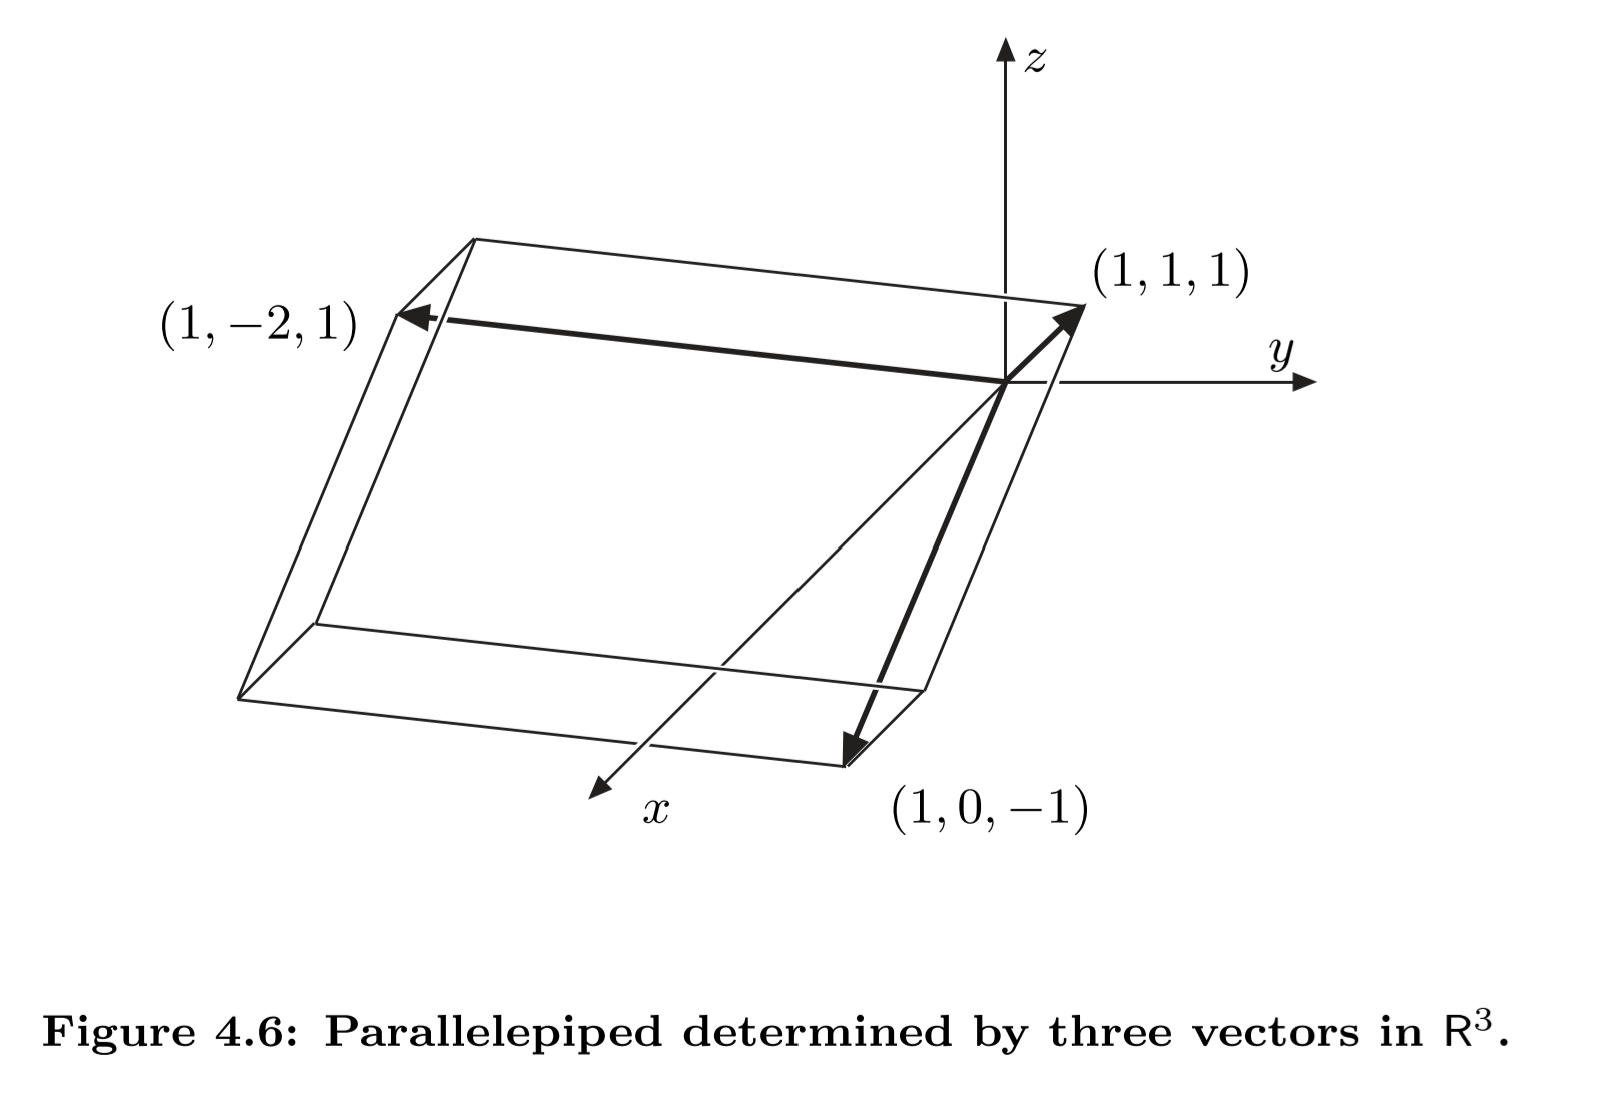
\includegraphics[width=16cm]{images/figure-4-6.png}

(BTW the figure doesn't look like a \emph{rectangular} parallelepiped.)

\begin{remark} \label{remark 4.3.4}
In our earlier discussion of the geometric significance of the determinant formed from the vectors in an ordered basis for \(\SET{R}^2\), we also saw that this determinant is positive if and only if the basis induces a \emph{right-handed coordinate system}.
(See \EXEC{4.1.13}.)
A similar statement is true in \(\SET{R}^n\).
\end{remark}

\begin{additional definition}
Specifically, if \(\gamma\) is any ordered basis for \(\SET{R}^{n}\)
and \(\beta\) is the \emph{standard} ordered basis for \(\SET{R}^n\), then \(\gamma\) induces a right-banded coordinate system if and only if \(\det(Q) > 0\), where \(Q\) is the \emph{change of coordinate matrix} that changes \(\gamma\)-coordinates into \(\beta\)-coordinates.
\end{additional definition}

Thus. for instance,
\[
    \gamma = \left\{
                \begin{pmatrix} 1 \\ 1 \\ 0 \end{pmatrix},
                \begin{pmatrix} 1 \\ -1 \\ 0 \end{pmatrix},
                \begin{pmatrix} 0 \\ 0 \\ 1 \end{pmatrix}
             \right\}
\]
induces a left-handed coordinate system in \(\SET{R}^3\) because the corresponding change of coordinate matrix (derived by \RMK{2.5.1} or \CORO{2.23.1})
\[
    \begin{pmatrix}
        1 & 1 & 0 \\
        1 & -1 & 0 \\
        0 & 0 & 1
    \end{pmatrix}
\]
has determinant \(-2 < 0\), whereas
\[
    \gamma' = \left\{
                \begin{pmatrix} 1 \\ 2 \\ 0 \end{pmatrix},
                \begin{pmatrix} -2 \\ 1 \\ 0 \end{pmatrix},
                \begin{pmatrix} 0 \\ 0 \\ 1 \end{pmatrix}
             \right\}
\]
induces a right-handed coordinate system in \(\SET{R}^3\) because the change of coordinate matrix (again derived by \RMK{2.5.1} or \CORO{2.23.1})
\[
    \begin{pmatrix}
        1 & -2 & 0 \\
        2 & 1 & 0 \\
        0 & 0 & 1
    \end{pmatrix}
\]
has determinant \(5 > 0\).

More generally, if \(\beta\) and \(\gamma\) are two ordered bases for \(\SET{R}^n\), then the coordinate systems induced by \(\beta\) and \(\alpha\) have the \emph{same orientation} (either both are right-handed or both are left-handed)
if and only if \(\det(Q) > 0\), where \(Q\) is the change of coordinate matrix that changes \(\gamma\)-coordinates into \(\beta\)-coordinates.

\exercisesection

\begin{exercise} \label{exercise 4.3.1}
Label the following statements as true or false.
\begin{enumerate}
\item If \(E\) is an elementary matrix, then \(\det(E) = \pm 1\).
\item For any \(A, B \in M_{n \X n}(F)\), \(\det(AB) = \det(A) \cdot \det(B)\).
\item A matrix \(M \in M_{n \X n}(F)\) is invertible if and only if \(\det(M) = 0\).
\item A matrix \(M \in M_{n \X n}(F)\) has rank \(n\) if and only if \(\det(M) \ne 0\).
\item For any \(A \in M_{n \X n}(F)\), \(\det(A^\top) = -\det(A)\).
\item The determinant of a square matrix can be evaluated by cofactor expansion along any \emph{column}.
\item Every system of \(n\) linear equations in \(n\) unknowns can be solved by Cramer's rule.
\item Let \(Ax = b\) be the matrix form of a system of \(n\) linear equations in \(n\) unknowns, where \(x = (x_1, x_2, ..., x_n)^\top\).
If \(\det(A) \ne 0\) and if \(M_k\) is the \(n \X n\) matrix obtained from \(A\) by replacing \RED{row} \(k\) of \(A\) by \(b^\top\), then the unique solution of \(Ax = b\) is
\[
    x_k = \cfrac{\det(M_k)}{\det(A)} \text{ for } k = 1, 2, ..., n.
\]
\end{enumerate}
\end{exercise}

\begin{proof} \ 

\begin{enumerate}
\item False. Type 2 with scalar \(c\) has determinant \(c\).
\item True by \THM{4.7}.
\item False by \CORO{4.7.1}.
\item True. \(M\) has rank \(n\), iff (by \RMK{3.2.1}) \(M\) is invertible, iff (by \CORO{4.7.1}) \(\det(M) \ne 0\).
\item False by \THM{4.8}.
\item True.
    We have \(\det(A) = \det(A^\top)\) by \THM{4.8}.
    And (by \THM{4.4}) \(\det(A^\top)\) is equal to the cofactor expansion along any \emph{row} of \(A^\top\).
    But that is equivalent to the cofactor expansion along any \(\emph{column}\) of \(A\).
\item False.
    The corresponding coefficient matrix also needs to be invertible.
\item False. By \THM{4.9}, \(M_k\) should be the \(n \X n\) matrix obtained from \(A\) by replacing \RED{column} \(k\) of \(A\) by \(b^\top\).
\end{enumerate}
\end{proof}

\begin{exercise} \label{exercise 4.3.2}
Solve the system using Cramer's rule:
\begin{align*}
    a_{11} x_1 + a_{12} x_2 & = b_1 \\
    a_{21} x_1 + a_{22} x_2 & = b_2
\end{align*}
where \(a_{11} a_{22} - a_{12} a_{21} \ne 0\).
\end{exercise}

\begin{proof}
By the given supposition, the corresponding coefficient matrix of the system
\[
    A = \begin{pmatrix} a_{11} & a_{12} \\ a_{21} & a_{22} \end{pmatrix}
\]
has nonzero determinant.
So using \THM{4.9} Cramer's rule,
\[
    M_1 = \begin{pmatrix} b_1 & a_{12} \\ b_2 & a_{22} \end{pmatrix}, \quad
    M_2 = \begin{pmatrix} a_{11} & b_1 \\ a_{21} & b_2 \end{pmatrix},
\]
and
\[
    x_1 = \cfrac{\det(M_1)}{\det(A)} = \cfrac{b_1 a_{22} - a_{12} b_2}{a_{11} a_{22} - a_{12} a_{21}},
    \quad
    x_2 = \cfrac{\det(M_2)}{\det(A)} = \cfrac{a_{11} b_2 - b_1 a_{21}}{a_{11} a_{22} - a_{12} a_{21}}
\]
\end{proof}

Exercise 3 to Exercise 7 are pure calculation problems that require solving systems using Cramer's rule. Skip.

\setcounter{exercise}{7}
\begin{exercise} \label{exercise 4.3.8}
Use \THM{4.8} to prove a result analogous to \THM{4.3}, but for columns.
\end{exercise}

\begin{proof}
Let \(A \in M_{n \X n}(F)\) such that
\[
    A = \begin{pmatrix} a_1 & a_2 & ... & a_r & ... & a_n
    \end{pmatrix},
\]
where \(a_1, ..., a_n \in F^n\) are columns of \(A\).
Now let \(a_r = u + kv\) for some \(u, v \in F^n\) and scalar \(k\), and let \(B, C\) be the same as \(A\) except for replacing row \(r\) with \(u\) and \(v\), respectively.

Then we need to show \(\det(A) = \det(B) + k \cdot \det(C)\).
Then
\begin{align*}
    \det(A) & = \det(A^\top) & \text{by \THM{4.8}} \\
            & = \det \begin{pmatrix} a_1^\top \\ \vdots \\ a_r^\top \\ \vdots \\ a_n^\top \end{pmatrix} = \det \begin{pmatrix} a_1^\top \\ \vdots \\ u^\top + k \cdot v^\top \\ \vdots \\ a_n^\top \end{pmatrix} & \text{of course} \\
            & = \det \begin{pmatrix} a_1^\top \\ \vdots \\ u^\top \\ \vdots \\ a_n^\top \end{pmatrix} + k \cdot \det \begin{pmatrix} a_1^\top \\ \vdots \\ v^\top \\ \vdots \\ a_n^\top \end{pmatrix} & \text{by \THM{4.3}} \\
            & = \det(B^\top) + k \cdot \det(C^\top) & \text{of course} \\
            & = \det(B) + k \cdot \det(C), & \text{by \THM{4.8}}
\end{align*}
as desired.
\end{proof}

\begin{exercise} \label{exercise 4.3.9}
Prove that an \emph{upper triangular} \(n \X n\) matrix is invertible if and only if all its diagonal entries are nonzero.
\end{exercise}

\begin{proof}
An \emph{upper triangular} \(n \X n\) matrix is invertible, iff (by \CORO{4.7.1}) its determinant is nonzero, iff (by \EXEC{4.2.23}) the product of its diagonal entries are nonzero, iff (of course) all its diagonal entries are nonzero.
\end{proof}

\begin{exercise} \label{exercise 4.3.10}
A matrix \(M \in M_{n \X n}(F)\) is called \href{https://www.wikiwand.com/en/Nilpotent_matrix}{nilpotent} if, for some \emph{positive} integer \(k\), \(M^k = O\), where \(O\) is the \(n \X n\) zero matrix.
Prove that if \(M\) is nilpotent, then \(\det(M) = 0\).
\end{exercise}

\begin{note}
Concept-related exercise: \EXEC{2.3.16}(b).
\end{note}

\begin{proof}
We have
\begin{align*}
             & M^k = O \\
    \implies & \det(M^k) = \det(O) = 0 & \text{of course} \\
    \implies & \det(M)^k = 0 & \text{by \THM{4.7}} \\
    \implies & \det(M) = 0 & \text{of course}
\end{align*}
\end{proof}

\begin{exercise} \label{exercise 4.3.11}
A matrix \(M \in M_{n \X n}(\SET{C})\) is called \textbf{skew-symmetric} if \(M^\top = -M\).
Prove that if \(M\) is skew-symmetric and \(n\) is odd, then \(M\) is not invertible.
What happens if \(n\) is even?
\end{exercise}

\begin{note}
The complex number has characteristic \(0 \ne 2\).
The exercise would not apply if the field of the matrix has characteristic equal to \(2\).
\end{note}

\begin{proof}
By \EXEC{4.2.25}, we have \(\det(-M) = (-1)^n \det(M)\).
And by \THM{4.8}, we have \(\det(M^\top) = \det(M)\).
And by supposition \(-M = M^\top\), so we have \((-1)^n \det(M) = \det(M)\).
If \(n\) is odd, the equation implies \(-1 \det(M) = \det(M)\).
Which implies \(\det(M) = 0 \in \SET{C}\).
If \(n\) is even, then that only implies \(\det(M) = \det(M)\), hence we cannot conclude anything.
For example, (the skew-symmetric matrix) \(\begin{pmatrix} 0 & 1 \\ -1 & 0 \end{pmatrix}\) is invertible, but (the skew-symmetric matrix) \(O_{2 \X 2}\) is not invertible.
\end{proof}

\begin{exercise} \label{exercise 4.3.12}
A matrix \(Q \in M_{n \X n}(\SET{R})\) is called \textbf{orthogonal} if \(QQ^\top = I\).
Prove that if \(Q\) is orthogonal, then \(\det(Q) = \pm 1\).
\end{exercise}

\begin{note}
This exercise should be related to \CH{6}.
\end{note}

\begin{proof}
We have
\begin{align*}
    1 = \det(I) & = \det(QQ^\top) & \text{by supposition} \\
                & = \det(Q) \det(Q^\top) & \text{by \THM{4.7}} \\
                & = \det(Q) \det(Q), & \text{by \THM{4.8}} \\
\end{align*}
which implies \(\det(Q) = \pm 1\).
\end{proof}

\begin{exercise} \label{exercise 4.3.13}
For \(M \in M_{n \X n}(\SET{C})\), let \(\conjugatet{M}\) be the matrix such that \((\conjugatet{M})_{ij} = \conjugatet{M_{ij}}\) for all \(i, j\),
where \(\conjugatet{M_{ij}}\) is the complex conjugate of \(M_{ij}\).
\begin{enumerate}
\item Prove that \(\det(\conjugatet{M}) = \conjugatet{\det(M)}\).

\item A matrix \(Q \in M_{n \X n}(\SET{C})\) is called \textbf{unitary} if \(QQ^* = I\), where \(Q^* = \conjugatet{Q^\top}\).
Prove that if \(Q\) is a \emph{unitary} matrix, then \(\left| \det(Q) \right| = 1\).
\end{enumerate}
\end{exercise}

\begin{proof} \ 

\begin{enumerate}
\item We prove by induction on \(n\).
For \(n = 1\),
\begin{align*}
    \det(\conjugatet{M}) & = (\conjugatet{M})_{11} & \text{by \DEF{4.2} for dimension \(= 1\)} \\
                         & = \conjugatet{M_{11}} & \text{by supposition} \\
                         & = \conjugatet{\det(M)} & \text{by \DEF{4.2} for dimension \(= 1\)}
\end{align*}

Suppose inductively \(\det(\conjugatet{M}) = \conjugatet{\det(M)}\) for arbitrary \(M \in M_{k \X k}(\SET{C})\) such that \((\conjugatet{M})_{ij} = \conjugatet{M_{ij}}\) for all \(i, j\).
We have to show \(\det(\conjugatet{M}) = \conjugatet{\det(M)}\) for arbitrary \(M \in M_{(k + 1) \X (k + 1)}(\SET{C})\) such that \((\conjugatet{M})_{ij} = \conjugatet{M_{ij}}\) for all \(i, j\).
Then
\begin{align*}
    \det(\conjugatet{M}) & = \sum_{j = 1}^{(k + 1)} (\conjugatet{M})_{1j} \cdot (-1)^{1 + j} \cdot \det(\widetilde{(\conjugatet{M})}_{1j}) & \text{by \DEF{4.2}} \\
                         & = \sum_{j = 1}^{(k + 1)} \RED{\conjugatet{M_{1j}}} \cdot (-1)^{1 + j} \cdot \det(\widetilde{(\conjugatet{M})}_{1j}) & \text{by supposition} \\
                         & = \sum_{j = 1}^{(k + 1)} \conjugatet{M_{1j}} \cdot (-1)^{1 + j} \cdot \RED{\conjugatet{\det(\tilde{M}_{1j})}} & \text{by inductive hypothesis} \\
                         & = \sum_{j = 1}^{(k + 1)} \conjugatet{M_{1j} \cdot (-1)^{1 + j}} \cdot \conjugatet{\det(\tilde{M}_{1j})} & \text{of course (see theorem D.2(c)(e))} \\
                         & = \sum_{j = 1}^{(k + 1)} \conjugatet{M_{1j} \cdot (-1)^{1 + j} \cdot \det(\tilde{M}_{1j})} & \text{of course (see theorem D.2)(c)} \\
                         \\
                         & = \conjugatet{\sum_{j = 1}^{(k + 1)} M_{1j} \cdot (-1)^{1 + j} \cdot \det(\tilde{M}_{1j})} & \text{of course (see theorem D.2)(b)} \\
                         & = \conjugatet{\det(M)} & \text{by \DEF{4.2}}
\end{align*}

\item We have
\begin{align*}
    1 = \det(I) & = \det(QQ^*) & \text{by supposition} \\
                & = \det(Q) \det(Q^*) & \text{by \THM{4.7}} \\
                & = \det(Q) \det(\conjugatet{Q^\top}) & \text{by definition} \\
                & = \det(Q) \conjugatet{\det(Q^\top)} & \text{by part(a)} \\
                & = \det(Q) \conjugatet{\det(Q)} & \text{by \THM{4.8}} \\
                & = \abs{\det(Q)}^2, & \text{by definition in page 551}
\end{align*}
which implies \(\abs{\det(Q)} = 1\).
\end{enumerate}
\end{proof}

\begin{exercise} \label{exercise 4.3.14}
Let \(\beta = \{ u_1, u_2, ..., u_n \}\) be a subset of \(F^n\) containing \(n\) distinct vectors, and let \(B\) be the matrix in \(M_{n \X n}(F)\) having \(u_j\) as column \(j\).
Prove that \(\beta\) is a basis for \(F^n\) if and only if \(\det(B) \ne 0\).
\end{exercise}

\begin{proof}
We have \(\beta\) is a basis for \(F^n\) iff (by \CH{3}) \(\rank(B) = n\), iff (by \EXEC{4.3.1}(d)) \(\det(B) \ne 0\).
\end{proof}

\begin{exercise} \label{exercise 4.3.15}
Prove that if \(A, B \in M_{n \X n}(F)\) are \emph{similar}, then \(\det(A) = \det(B)\).
\end{exercise}

\begin{proof}
If \(A, B \in M_{n \X n}(F)\) are similar, then by \DEF{2.16} we have \(B = Q^{-1} A Q\) for some invertible \(Q\).
And
\begin{align*}
    \det(B) & = \det(Q^{-1} A Q) \\
            & = \det(Q^{-1}) \det(A) \det(Q) & \text{by \THM{4.7}} \\
            & = \det(Q^{-1}) \det(Q) \det(A) & \text{of course} \\
            & = \det(Q^{-1} Q) \det(A) & \text{by \THM{4.7}} \\
            & = \det(I) \det(A) & \text{of course} \\
            & = 1 \cdot \det(A) = \det(A) & \text{of course}
\end{align*}
\end{proof}

\begin{exercise} \label{exercise 4.3.16}
Use determinants to prove that if \(A, B \in M_{n \X n}(F)\) are such that \(AB = I\), then \(A\) is invertible (and hence \(B = A^{-1}\)).
\end{exercise}

\begin{note}
This is related to \ATHM{2.38}.
\end{note}

\begin{proof}
We have
\begin{align*}
    1 = \det(I) & = \det(AB) & \text{by supposition} \\
                & = \det(A) \det(B), & \text{by \THM{4.7}}
\end{align*}
which implies both \(\det(A)\) and \(\det(B)\) cannot be zero.
And in particular by \CORO{4.7.1}, \(A\) is invertible.
And by \ATHM{2.38}(1), \(B = A^{-1}\).
\end{proof}

\begin{exercise} \label{exercise 4.3.17}
Let \(A, B \in M_{n \X n}(F)\) be such that \(AB = -BA\).
Prove that if \(n\) is odd and \(F\) is \emph{not} a field of characteristic two, then \(A\) or \(B\) is not invertible.
\end{exercise}

\begin{proof}
We have
\begin{align*}
    \det(A) \det(B) & = \det(AB) & \text{by \THM{4.7}} \\
                    & = \det(-BA) & \text{by supposition} \\
                    & = (-1)^n \cdot \det(BA) & \text{by \EXEC{4.2.25}} \\
                    & = (-1) \cdot \det(BA) & \text{since \(n\) is odd} \\
                    & = -1 \cdot \det(B) \det(A) & \text{by \THM{4.7}} \\
                    & = -1 \cdot \det(A) \det(B) & \text{of course} \\
    \implies 2 \cdot \det(A) \det(B) = 0.
\end{align*}
Since \(F\) is \emph{not} a field of characteristic two, that implies \(\det(A) \det(B) = 0\), so \(\det(A)\) \emph{or} \(\det(B)\) is zero, so by \CORO{4.7.1}, \(A\) or \(B\) is not invertible.
\end{proof}

\begin{exercise} \label{exercise 4.3.18}
Complete the proof of \THM{4.7} by showing that if \(A\) is an \emph{elementary matrix} of type 2 or type 3, then \(\det(AB) = \det(A) \cdot \det(B)\).
\end{exercise}

\begin{proof}
If \(A\) is type 2, then \(A\) has the form
\[
    A = \begin{pmatrix}
        e_1 \\ e_2 \\ \vdots \\ k e_i \\ \vdots \\ e_n
    \end{pmatrix}
\]
where \(k\) is nonzero scalar.
And by \THM{3.1}, \(AB\) is equal to \(B\) with row \(i\) multiplied by \(k\), so by \RMK{4.2.3}(b), \(\det(AB) = k \cdot \det(B)\) \MAROON{(1)}.
And by \RMK{4.3.1}, \(\det(A) = k\), hence by \MAROON{(1)} we have \(\det(AB) = \det(A) \cdot \det(B)\).

If \(A\) is type 3, then \(A\) has the form
\[
    A = \begin{pmatrix}
        e_1 \\ e_2 \\ \vdots \\ k e_i + e_j \\ \vdots \\ e_n
    \end{pmatrix}
\]
And by \THM{3.1}, \(AB\) is equal to \(B\) but adding \(k\) times row \(i\) to row \(j\), so by \RMK{4.2.3}(c), \(\det(AB) = \det(B)\) \MAROON{(2)}.
And by \RMK{4.3.1}, \(\det(A) = 1\), hence by \MAROON{(2)} we have \(\det(AB) = \det(B) = 1 \cdot \det(B) = \det(A) \cdot \det(B)\).
\end{proof}

\begin{exercise} \label{exercise 4.3.19}
A matrix \(A \in M_{n \X n}(F)\) is called \textbf{lower triangular} if \(A_{ij} = 0\) for \(1 \le i < j \le n\).
Suppose that \(A\) is a lower triangular matrix.
Describe \(\det(A)\) in terms of the entries of \(A\).
\end{exercise}

\begin{proof}
If \(A\) is lower triangular, then \(A^\top\) is upper triangular.
By \THM{4.8}, \(\det(A) = \det(A^\top)\).
And by \EXEC{4.2.23}, we know \(\det(A^\top)\) is equal to the product of its diagonals, so \(\det(A)\) is equal to the product of \(A^\top\)'s diagonals.
But \(A^\top\)'s diagonals are of course \(A\)'s diagonals, so \(\det(A)\) is also equal to the product of its diagonals.
\end{proof}

\begin{exercise} \label{exercise 4.3.20}
Suppose that \(M \in M_{n \X n}(F)\) can be written in the form
\[
    M = \begin{pmatrix} A & B \\ O & I \end{pmatrix},
\]
where \(A\) is a \emph{square} matrix.
Prove that \(\det(M) = \det(A)\).
\end{exercise}

\begin{proof}
Informally, if we expand the last row of \(M\), then ultimately we have
\[
    \det(M) = 1 \cdot 1 \cdot ... \cdot 1 \cdot \det(A) = \det(A).
\]
\end{proof}

\begin{exercise} \label{exercise 4.3.21}
Prove that if \(M \in M_{n \X n}(F)\) can be written in the form
\[
    M = \begin{pmatrix} A & B \\ O & C \end{pmatrix},
\]
where \(A\) and \(C\) are square matrices, then \(\det(M) = \det(A) \cdot \det(C)\).
\end{exercise}

\begin{proof}
There are two cases: \(C\) is invertible or not.

If \(C\) is not invertible, then the rows of \(C\) is \emph{not} \LID{}, and (by \CORO{4.7.1}) \(\det(C) = 0\);
and of course the rows of \((O|C)\) is not \LID{}, which implies \(M\) has rank less then \(n\), so (by \CORO{4.6.1}) \(\det(M) = 0\).
And \(\det(A) \cdot \det(C) = \det(A) \cdot 0 = 0\), hence \(\det(M) = \det(A) \cdot \det(C)\).

If \(C\) is invertible, then given the matrix
\[
    M' = \begin{pmatrix} I & O \\ O & C^{-1} \end{pmatrix},
    M'' = \begin{pmatrix} A & B \\ O & I \end{pmatrix},
\]
by (the generalization of) \ATHM{3.7},
\[
    M' M =
    \begin{pmatrix} I & O \\ O & C^{-1} \end{pmatrix}
    \begin{pmatrix} A & B \\ O & C \end{pmatrix}
    = M'',
\]
So we have \(\det(M' M) = \det(M'')\), so by \THM{4.7}, \(\det(M')\det(M) = \det(M'')\) \MAROON{(1)}.
By (similar argument of) \EXEC{4.3.20}, \(\det(M') = \det(C^{-1})\).
And by \EXEC{4.3.20}, \(\det(M'') = \det(A)\), so by \MAROON{(1)}, we have \(\det(C^{-1}) \det(M) = \det(A)\).
And by \CORO{4.7.1}, that implies
\[
    \cfrac{1}{\det(C)} \det(M) = \det(A), \text{ so } \det(M) = \det(A) \cdot \det(C).
\]
So in all cases, we have \(\det(M) = \det(A) \cdot \det(C)\).
\end{proof}

\begin{exercise} \label{exercise 4.3.22}
Let \(\T : \POLYNF \to F^{n + 1}\) be the \LTRAN{} defined in \EXEC{2.4.22} by \(\T(f) = (f(c_0), f(c_1), ..., f(c_n))\), where \(c_0, c_1, ..., c_n\) are \emph{distinct} scalars in an infinite field \(F\).
Let \(\beta\) be the \emph{standard} ordered basis for \(\POLYNF\) and \(\gamma\) be the \emph{standard} ordered basis for \(F^{n + 1}\).
\begin{enumerate}
\item Show that the \((n + 1) \X (n + 1)\) matrix \(M = [\T]_{\beta}^{\gamma}\) has the form
\[
    \begin{pmatrix}
        1 & c_0 & c_0^2 & ... & c_0^n \\\
        \vdots & \vdots & \vdots & & \vdots \\
        1 & c_{n-1} & c_{n-1}^2 & ... & c_{n-1}^n \\
        1 & c_n & c_n^2 & ... & c_n^n
    \end{pmatrix}
\]
A matrix with this form is called a \textbf{Vandermonde matrix}.
\item Use \EXEC{2.4.22} to prove that \(\det(M) \ne 0\).
\item Prove that
\[
    \det(M) = \prod_{0 \le i < j \le n} (c_j - c_i),
\]
the product of all terms of the form \(c_j - c_i\) for \(0 \le i < j \le n\).
\end{enumerate}
\end{exercise}

\begin{proof} \ 

\begin{enumerate}
\item
For the standard ordered base \(\beta = \{ 1, x, x^2, ..., x^n \}\), we have
\begin{align*}
    \T(1) & = (1, 1, ..., 1) = 1 \cdot e_1 + 1 \cdot e_2 + ... + 1 \cdot e_{n+1} \\
    \T(x) & = (c_0, c_1, ..., c_n) = c_0 \cdot e_1 + c_1 \cdot e_2 + ... + c_n \cdot e_{n+1} \\
    \T(x^2) & = (c_0^2, c_1^2, ..., c_n^2) = c_0^2 \cdot e_1 + c_1^2 \cdot e_2 + ... + c_n^2 \cdot e_{n+1} \\
    \vdots \\
    \T(x^n) & = (c_0^n, c_1^n, ..., c_n^n) = c_0^n \cdot e_1 + c_1^n \cdot e_2 + ... + c_n^n \cdot e_{n+1}
\end{align*}
So \([\T]_{\beta}^{\gamma}\) has that desired form.

\item \(\T\) is an isomorphism, so by \THM{2.18}, \(M = [\T]_{\beta}^{\gamma}\) is invertible, so by \CORO{4.7.1}, \(\det(M) \ne 0\).

\item Let
\[
    F_1 = \begin{pmatrix}
        1 & c_0 & c_0^2 & ... & c_0^n \\\
        \vdots & \vdots & \vdots & & \vdots \\
        1 & c_{n-1} & c_{n-1}^2 & ... & c_{n-1}^n \\
        1 & x & x^2 & ... & x^n
    \end{pmatrix}
    \quad \text{and } \quad
    f_1(x) = \det (F_1).
\]
Then its clear that, by expanding the last row of \(F_1\), \(f_1(x)\) is a polynomial of degree \(n\).
And in particular,
\[
    f_1(c_n) = \det(M) \quad \quad \MAROON{(1.1)}.
\]
Furthermore, \(c_0, c_1, ..., c_{n-1}\) are the \(n\) roots of this polynomial, since from the structure of \(F_1\), if we replace \(x\) with \(c_0, ..., c_{n - 1}\), then \(F_1\) has two identical rows, so (by \CORO{4.4.1}) the determinant is equal to zero.
So \(f_1(x)\) has the form
\[
    f_1(x) = \alpha_1 (x - c_0)(x - c_1) ... (x - c_{n - 1}), \quad \quad \MAROON{(1.2)}
\]
where \(\alpha_1\) is a nonzero scalar.
\textbf{But again}, from the structure of \(F_1\), \(\alpha_1\) is in fact equal to the cofactor of the row \(n + 1\), column \(n + 1\).
That is,
\[
    \alpha_1 = (-1)^{(n + 1) + (n + 1)} \det \left( \widetilde{F_1}_{(n+1)(n+1)} \right) = \det\left( \widetilde{F_1}_{(n+1)(n+1)} \right).
\]
\emph{That is},
\[
    \alpha_1 = \det \begin{pmatrix}
        1 & c_0 & c_0^2 & ... & c_0^{n \RED{- 1}} \\\
        \vdots & \vdots & \vdots & & \vdots \\
        1 & c_{n \RED{-1}} & c_{n \RED{-1}}^2 & ... & c_{n \RED{-1}}^{n \RED{- 1}}
    \end{pmatrix}. \quad \quad \MAROON{(1.3)}
\]
Now if we \textbf{use the same argument again}, then we let
\[
    F_2 = \begin{pmatrix}
        1 & c_0 & c_0^2 & ... & c_0^{n - 1} \\\
        \vdots & \vdots & \vdots & & \vdots \\
        1 & c_{n-2} & c_{n-2}^2 & ... & c_{n-2}^{n - 1} \\
        1 & x & x^2 & ... & x^{n-1}
    \end{pmatrix}
    \quad \text{and} \quad
    f_2(x) = \det(F_2).
\]
Then in particular, by observation,
\[
    f_2(c_{n - 1}) = \alpha_1 \quad \quad \MAROON{(2.1)}.
\]
Using the same argument, we have
\[
    f_2(x) = \alpha_2 (x - c_0)(x - c_1) ... (x - c_{n - 2}), \quad \quad \MAROON{(2.2)}
\]
where
\[
    \alpha_2 = \det \begin{pmatrix}
        1 & c_0 & c_0^2 & ... & c_0^{n \RED{- 2}} \\\
        \vdots & \vdots & \vdots & & \vdots \\
        1 & c_{n \RED{-2}} & c_{n \RED{-2}}^2 & ... & c_{n \RED{-2}}^{n \RED{- 2}}
    \end{pmatrix}. \quad \quad \MAROON{(2.3)}
\]

Continue this process \emph{inductively}, we have
\begin{align*}
    \det(M) & = f_1(c_n) & \text{by \MAROON{(1.1)}} \\
            & = \alpha_1 \cdot (c_n - c_0) (c_n - c_1) ... (c_n - c_{n - 1}) & \text{by \MAROON{(1.2)}} \\
            & = f_2(c_{n - 1}) \cdot [(c_n - c_0) (c_n - c_1) ... (c_n - c_{n - 1})] & \text{by \MAROON{(2.1)}} \\
            & = \big[ \alpha_2 (c_{n - 1} - c_0) (c_{n - 1} - c_1) ... (c_{n - 1} - c_{n - 2}) \big] \\
            & \quad \quad \cdot \big[ (c_n - c_0) (c_n - c_1) ... (c_n - c_{n - 1}) \big] & \text{by \MAROON{(2.2)}} \\
            & \quad \vdots \\
            & = \big[(c_1 - c_0)] \big[(c_2 - c_0) (c_2 - c_1) ] \\
            & \quad \quad \cdot ... \\
            & \quad \quad \cdot \big[ (c_{n - 1} - c_0) (c_{n - 1} - c_1) ... (c_{n - 1} - c_{n - 2}) \big] \\
            & \quad \quad \cdot \big[ (c_n - c_0) (c_n - c_1) ... (c_n - c_{n - 1}) \big] & \text{expand inductively} \\
            & = \prod_{0 \le i < j \le n} (c_j - c_i).
\end{align*}
\end{enumerate}
\end{proof}

\begin{exercise} \label{exercise 4.3.23}
Let \(A \in M_{n \X n}(F)\) be nonzero.
For any \(m\) (\(1 \le m \le n\)), an \(m \X m\) \textbf{submatrix} is obtained by deleting \emph{any} \(n - m\) rows and any \(n - m\) columns of \(A\).
(The concept is similar to a \emph{subsequence} of a sequence.)
\begin{enumerate}
\item Let \(k\) (\(1 \le k \le n\)) denote the \emph{largest} integer such that some \(k \X k\) submatrix has a nonzero determinant.
Prove that \(\rank(A) = k\).
\item Conversely, suppose that \(\rank(A) = k\).
Prove that there exists a \(k \X k\) submatrix with a nonzero determinant.
\end{enumerate}
\end{exercise}

\begin{proof} \ 

\begin{enumerate}
\item
If \(\rank(A) = n\), that means \(A\) is invertible, and by \CORO{4.7.1}, \(\det(A) \ne 0\).
So the largest submatrix with a nonzero determinant is \(A\) itself, which has size \(n \X n\), so in this case, \(k = n\), which is equal to \(\rank(A)\).

Now suppose \(\rank(A) < n\).
We will show that \(\rank(A) < k\) and \(\rank(A) > k\) lead to contradiction.

So for the sake of contradiction, suppose
\[
    \rank(A) < k. \quad \quad \BLUE{(1)}
\]
First let \(B\) be the \(k \X k\) submatrix of \(A\) with nonzero determinant.
Then by \CORO{4.7.1}, \(B\) is invertible, and the columns \(S = \{ v_1, v_2, ..., v_k \}\) of \(B\) are \LID{}.
Now consider the \(k \X \RED{n}\) submatrix \(C\) of \(A\) obtained by deleting those rows who were deleted when we construct \(B\).
Then \(S\) is a \emph{subset} of the columns of \(C\).
This means \(\rank(C) \ge \#S = k\).
But by \THM{3.6}, \(\rank(C) \le \min(k, n) = k\).
Hence \(\rank(C) = k\), which implies the \(k\) rows of \(C\) are also \LID{}.
And thus the matrix \(A\) contains these \(k\) \LID{} rows and hence \(\rank(A) \ge k\), which contradicts \BLUE{(1)}.

Now, for the sake of contradiction, suppose
\[
    \rank(A) > k. \quad \quad \BLUE{(2)}
\]
Let \(\rank(A) = r\).
Then we can pick \(r\) \LID{} rows of \(A\), say \(u_1, ..., u_r\), to construct a \(r \X n\) submatrix \(D\) of \(A\).
Then \(D\) has \(\rank(D) \ge r\).
And by \THM{3.6}, \(\rank(D) \le \min(r, n) = r\), hence \(\rank(D) = r\).
Now we can also pick \(r\) \LID{} \emph{columns}, say \(v_1, ..., v_r\), of \(D\), to construct an \(r \X r\) submatrix \(D'\) of \(D\).
Note that \(D'\) is also a submatrix of \(A\).
Then \(\rank(D') \ge r\), and again by \THM{3.6}, \(\rank(D') \le min(r, r) = r\), hence \(\rank(D') = r\).
This implies \(D'\) is invertible, and by \CORO{4.7.1}, \(\det(D') \ne 0\).
So we have found a \(r \X r\) submatrix of \(A\) with nonzero determinant and \(r > k\), which contradicts the property of \(k\) that \(k\) is the size of the ``largest'' nonzero determinant submatrix of \(A\).

So \(\rank(A)\) must be equal to \(k\).

\item This is similar to the second part of the proof in part(a),
We just pick \(k\) \LID{} rows of \(A\) to construct a \(k \X n\) submatrix, and pick \LID{} \(k\) columns of that submatrix to construct a \(k \X k\) submatrix.
Then such \(k \X k\) matrix is a submatrix of \(A\) and has nonzero determinant.
\end{enumerate}
\end{proof}

\begin{exercise} \label{exercise 4.3.24}
Let \(A \in M_{n \X n}(F)\) have the form
\[
    A = \left(\begin{array}{rrcccc}
        0 & 0 & 0 & \cdots & 0 & a_{0} \\
        -1 & 0 & 0 & \cdots & 0 & a_{1} \\
        0 & -1 & 0 & \cdots & 0 & a_{2} \\
        \vdots & \vdots & \vdots & \ddots & \vdots & \vdots \\
        0 & 0 & 0 & \cdots & 0 & a_{n-2} \\
        0 & 0 & 0 & \cdots & -1 & a_{n-1}
    \end{array}\right)
\]
Compute \(\det(A + tI)\), where \(I\) is the \(n \X n\) identity matrix.
\end{exercise}

\begin{proof}
\(A + tI\) has the form
\[
    \begin{pmatrix}
        t      & 0      & 0      & \cdots & 0      & a_{0} \\
        -1     & t      & 0      & \cdots & 0      & a_{1} \\
        0      & -1     & t      & \cdots & 0      & a_{2} \\
        \vdots & \vdots & \vdots & \ddots & \vdots & \vdots \\
        0      & 0      & 0      & \cdots & t      & a_{n-2} \\
        0      & 0      & 0      & \cdots & -1     & t + a_{n-1}
    \end{pmatrix}
\]
We perform type 3 elementary row operations:
\begin{align*}
    \begin{pmatrix}
        t      & 0      & 0      & \cdots & 0      & a_{0} \\
        -1     & t      & 0      & \cdots & 0      & a_{1} \\
        0      & -1     & t      & \cdots & 0      & a_{2} \\
        \vdots & \vdots & \vdots & \ddots & \vdots & \vdots \\
        0      & 0      & 0      & \cdots & t      & a_{n-2} \\
        0      & 0      & 0      & \cdots & -1     & t + a_{n-1}  
    \end{pmatrix}
    \to
    \begin{pmatrix}
        t       & 0      & 0      & \cdots & 0      & a_{0} \\
        \RED{0} & t      & 0      & \cdots & 0      & \RED{a_{1} + \cfrac{a_0}{t}} \\
        0       & -1     & t      & \cdots & 0      & a_{2} \\
        \vdots  & \vdots & \vdots & \ddots & \vdots & \vdots \\
        0      & 0      & 0      & \cdots & t      & a_{n-2} \\
        0       & 0      & 0      & \cdots & -1     & t + a_{n-1}  
    \end{pmatrix} \\
    \to
    \begin{pmatrix}
        t       & 0       & 0      & \cdots & 0      & a_{0} \\
        0       & t       & 0      & \cdots & 0      & a_{1} + \cfrac{a_0}{t} \\
        0       & \RED{0} & t      & \cdots & 0      & \RED{a_{2} + \cfrac{a_{1}}{t} + \cfrac{a_0}{t^2}} \\
        \vdots  & \vdots  & \vdots & \ddots & \vdots & \vdots \\
        0       & 0       & 0      & \cdots & t      & a_{n-2} \\
        0       & 0       & 0      & \cdots & -1     & t + a_{n-1}   
    \end{pmatrix}
    \to ... \to
    \begin{pmatrix}
        t       & 0       & 0      & \cdots & 0       & a_{0} \\
        0       & t       & 0      & \cdots & 0       & a_{1} + \cfrac{a_0}{t} \\
        0       & 0       & t      & \cdots & 0       & a_{2} + \cfrac{a_{1}}{t} + \cfrac{a_0}{t^2} \\
        \vdots  & \vdots  & \vdots & \ddots & \vdots  & \vdots \\
        0       & 0       & 0      & \cdots & t       & \vdots \\
        0       & 0       & 0      & \cdots & \RED{0} & \RED{t + a_{n-1} + \cfrac{a_{n-2}}{t} + ... + \cfrac{a_0}{t^{n-1}}}
    \end{pmatrix}
\end{align*}
which is upper triangular.
So by \EXEC{4.2.23}, the determinant is equal to the product of the diagonal entries, that is
\[
    t^{n - 1} (t + a_{n-1} + \cfrac{a_{n-2}}{t} + ... + \cfrac{a_0}{t^{n-1}})
    = t^n + t^{n - 1} a_{n - 1} + t^{n - 2} a_{n - 2} + ... + t a_1 + a_0.
\]
So \(\det(A) = t^n + t^{n - 1} a_{n - 1} + t^{n - 2} a_{n - 2} + ... + t a_1 + a_0\).
\end{proof}

\begin{exercise} \label{exercise 4.3.25}
Let \(c_{jk}\) denote the cofactor (see \DEF{4.2}) of the row \(j\), column \(k\) entry of the matrix \(A \in M_{n \X n}(F)\).
\begin{enumerate}
\item Prove that if \(B\) is the matrix obtained from \(A\) by replacing \emph{column} \(k\) by \(e_j\), then \(\det(B) = c_{jk}\).

\item Show that for \(1 \le j \le n\), we have
\[
    A \begin{pmatrix} c_{j1} \\ c_{j2} \\ \vdots \\ c_{jn} \end{pmatrix}
    = \det(A) \cdot e_j.
\]
Hint: Apply Cramer's rule to \(Ax = e_j\).

\item Deduce that if \(C\) is the \(n \X n\) matrix such that \(C_{ij} = c_{\RED{ji}}\), then \(AC = [\det(A)]I\).
(Notice the order of the suffix.)

\item Show that if \(\det(A) \ne 0\), then \(A^{-1} = [\det(A)]^{-1}C\).
\end{enumerate}
\end{exercise}

\begin{proof} \ 

\begin{enumerate}
\item Just expanding the column \(k\) of \(B\):
\begin{align*}
    \det(B) & = \sum_{i = 1}^n B_{ik} \cdot (-1)^{i + k} \det(\tilde{B}_{ik}) \\
            & = \sum_{i = 1}^n A_{ik} \cdot (-1)^{i + k} \det(\tilde{B}_{ik}) & \text{since \(A, B\) only differ in column \(k\)} \\
            & = \sum_{i = 1}^n B_{ik} \cdot c_{ik} & \text{by def of cofactor} \\
            & = 0 \cdot c_{1k} + ... + 1 \cdot c_{jk} + ... + 0 \cdot c_{nk} & \text{since column \(k\) of \(B = e_j\)} \\
            & = c_{jk}.
\end{align*}

\item We just check each entry of the product.
The product is
\begin{equation} \label{exec.4.3.25.eq}
    A \begin{pmatrix} c_{j1} \\ c_{j2} \\ \vdots \\ c_{jn} \end{pmatrix}
    = \begin{pmatrix}
        A_{11} c_{j1} + ... + A_{1n} c_{jn} \\
        A_{21} c_{j1} + ... + A_{2n} c_{jn} \\
        \vdots \\
        \RED{A_{j1} c_{j1} + ... + A_{jn} c_{jn}} \\
        \vdots \\
        A_{n1} c_{j1} + ... + A_{nn} c_{jn}
    \end{pmatrix}
    = \begin{pmatrix}
        \sum_{k = 1}^n A_{1k} c_{jk} \\
        \sum_{k = 1}^n A_{2k} c_{jk} \\
        \vdots \\
        \RED{\det(A)} \\
        \vdots \\
        \sum_{k = 1}^n A_{nk} c_{jk}
    \end{pmatrix}
\end{equation}
For the \(i\)th entry of the product where \(i \ne j\), it can be seen as the cofactor expansion of \(B_i\) that is obtained by replacing the \(j\)th row of \(A\) with the \(i\)th row of \(A\);
that is,
\[
    B_i = \begin{blockarray}{cccc}
        \begin{block}{(ccc)c}
        A_{11} & ... & A_{1n} & \\
        \vdots &     & \vdots & \\
        A_{i1} & ... & A_{in} & \RED{i} \\
        \vdots &     & \vdots & \\
        \RED{A_{i1}} & \RED{...} & \RED{A_{in}} & \RED{j}\\
        \vdots &     & \vdots & \\
        A_{n1} & ... & A_{nn} & \\
        \end{block}
    \end{blockarray}
\]
Since \(B_i\) has two identical rows, by \CORO{4.4.1}, \(\det(B_i) = 0\);
that is, the \(i\)th entry, where \(i \ne j\), of the product in \ref{exec.4.3.25.eq} is zero.
Hence
\[
    A \begin{pmatrix} c_{j1} \\ c_{j2} \\ \vdots \\ c_{jn} \end{pmatrix} = \begin{pmatrix}
        0 \\ \vdots \\ \det(A) \\ \vdots \\ 0
    \end{pmatrix} = \det(A) \cdot e_j.
\]

\item By the previous exercise
\begin{align*}
    AC & = A \begin{pmatrix}
            c_{11} & c_{21} & ... & c_{n1} \\
            c_{12} & c_{22} & ... & c_{n2} \\
            \vdots & \vdots &     & \vdots \\
            c_{1n} & c_{2n} & ... & c_{nn}
           \end{pmatrix} \\
       & = \begin{pmatrix}
           A \begin{pmatrix} c_{11} \\ c_{12} \\ \vdots \\ c_{1n} \end{pmatrix}
           & A \begin{pmatrix} c_{21} \\ c_{22} \\ \vdots \\ c_{2n} \end{pmatrix}
           & ...
           & A \begin{pmatrix} c_{n1} \\ c_{n2} \\ \vdots \\ c_{nn} \end{pmatrix}
       \end{pmatrix} & \text{by \THM{2.13}(a)} \\
       & = \begin{pmatrix}
           \det(A) e_1 & \det(A) e_2 & ... & \det(A) e_n
       \end{pmatrix} & \text{by part(b)} \\
       & = \det(A) \begin{pmatrix} e_1 & e_2 & ... & e_n \end{pmatrix} = \det(A) \cdot I & \text{of course}
\end{align*}
In fact the matrix \(C\) is called the classical adjoint matrix of \(A\), see \ADEF{4.4} below.

\item If \(\det(A) \ne 0\), then by \CORO{4.7.1}, \(A\) is invertible.
And
\begin{align*}
             & AC = \det(A) \cdot I & \text{by part(c)} \\
    \implies & A^{-1} AC = A^{-1} (\det(A) \cdot I) \\
    \implies & C = \det(A) \cdot A^{-1} I \\
    \implies & C = \det(A) \cdot A^{-1} \\
    \implies & [\det(A)]^{-1} C = A^{-1}
\end{align*}
\end{enumerate}
\end{proof}

\begin{additional definition} \label{adef 4.4}
The \textbf{classical adjoint} of a square matrix \(A\) is the \emph{transpose} of the matrix whose \(ij\)-entry is the \(ij\)-cofactor of \(A\).
That is, the \(ij\)-entry of the classical adjoint is the \(ji\)-cofactor of \(A\).
\end{additional definition}

\begin{exercise} \label{exercise 4.3.26}
Find the classical adjoint of each of the following matrices.

(a) \(\left(\begin{array}{ll}A_{11} & A_{12} \\ A_{21} & A_{22}\end{array}\right)\)
(b) \(\left(\begin{array}{lll}4 & 0 & 0 \\ 0 & 4 & 0 \\ 0 & 0 & 4\end{array}\right)\)

(c) \(\left(\begin{array}{rrr}-4 & 0 & 0 \\ 0 & 2 & 0 \\ 0 & 0 & 5\end{array}\right)\)
(d) \(\left(\begin{array}{lll}3 & 6 & 7 \\ 0 & 4 & 8 \\ 0 & 0 & 5\end{array}\right)\)

(e) \(\left(\begin{array}{ccc}1-i & 0 & 0 \\ 4 & 3 i & 0 \\ 2 i & 1+4 i & -1\end{array}\right)\)
(f) \(\left(\begin{array}{rrr}7 & 1 & 4 \\ 6 & -3 & 0 \\ -3 & 5 & -2\end{array}\right)\)

(g) \(\left(\begin{array}{rrr}-1 & 2 & 5 \\ 8 & 0 & -3 \\ 4 & 6 & 1\end{array}\right)\)
(h) \(\left(\begin{array}{ccc}3 & 2+i & 0 \\ -1+i & 0 & i \\ 0 & 1 & 3-2 i\end{array}\right)\)
\end{exercise}

\begin{proof} \ 

\begin{enumerate}
\item The adjoint matrix is
\begin{align*}
    \begin{pmatrix} c_{11} & c_{12} \\ c_{21} & c_{22} \end{pmatrix}^\top
        & = \begin{pmatrix} A_{22} & -A_{21} \\ -A_{12} & A_{11} \end{pmatrix}^\top \\
        & = \begin{pmatrix} A_{22} & -A_{12} \\ -A_{21} & A_{11} \end{pmatrix}
\end{align*}

\item The adjoint matrix is
\begin{align*}
    \begin{pmatrix} c_{11} & c_{12} & c_{13} \\ c_{21} & c_{22} & c_{23} \\ c_{31} & c_{32} & c_{33} \end{pmatrix}^\top
        & = \begin{pmatrix} 16 & 0 & 0 \\ 0 & 16 & 0 \\ 0 & 0 & 16 \end{pmatrix}^\top \\
        & = \begin{pmatrix} 16 & 0 & 0 \\ 0 & 16 & 0 \\ 0 & 0 & 16 \end{pmatrix}
\end{align*}
\end{enumerate}

Skip the remaining items.
\end{proof}

\begin{exercise} \label{exercise 4.3.27}
Let \(C\) be the classical adjoint of \(A \in M_{n \X n}(F)\).
Prove the following statements.
\begin{enumerate}
\item \(\det(C) = [\det(A)]^{n-1}\).
\item \(C^\top\) is the classical adjoint of \(A^\top\).
\item If \(A\) is an invertible upper triangular matrix, then \(C\) and \(A^{-1}\) are both upper triangular matrices.
\end{enumerate}
\end{exercise}

\begin{note}
It seems that \(n\) should be at least \(\ge 2\), otherwise the classical adjoint matrix is not well-defined.
\end{note}

\begin{proof}
If \(A = O_{n \X n}\), then it's trivial to prove (a)(b) and (c) does not apply.
So suppose \(A \ne O_{n \X n}\).

\begin{enumerate}
\item If \(A\) is not invertible, then
\begin{align*}
    AC & = [\det(A)] I & \text{by \EXEC{4.3.25}(c)} \\
       & = 0 \cdot I = O_{n \X n}.
\end{align*}
Then \(C\) cannot be invertible, otherwise we have \(AC C^{-1} = O_{n \X n} C^{-1} = O_{n \X n} \implies A = O_{n \X n}\).
So \(\det(C) = 0\).
Then clearly \(\det(C) = 0 = 0^{n - 1} = [\det(A)]^{n - 1}\).

If \(A\) is invertible, then
\begin{align*}
             & \det(AC) = \det([\det(A)]I) & \text{by \EXEC{4.3.25}(c)} \\
    \implies & \det(A)\det(C) = \det([\det(A)]I) & \text{by \THM{4.7}} \\
    \implies & \det(A)\det(C) = [\det(A)]^n \cdot \det(I) & \text{by \EXEC{4.2.25}} \\
    \implies & \det(C) = \det(A)^{n - 1} & \text{of course}
\end{align*}
So in all cases we have \(\det(C) = \det(A)^{n - 1}\).

\item
Let \(c_{ij}\) be the \(ij\)-cofactor of \(A\).

First, by \ADEF{4.4}, since \(C\) is the \emph{transpose} of the matrix whose \(ij\)-entry is the \(ij\)-cofactor of \(A\), that implies the \(ij\)-entry of \(C^\top\) is just the \(ij\)-cofactor of \(A\).
That is,
\[
    (C^\top)_{ij} = c_{ij} = (-1)^{i + j} \det(\tilde{A}_{ij}).
\]
But by \THM{4.8}, \(\det(\tilde{A}_{ij}) = \det((\widetilde{A}_{ij})^\top)\), which is equal to \(\det((\widetilde{A^\top})_{ji} )\).
(Removing row \(i\), column \(j\) then taking transpose is equal to taking transpose then remove row \(j\) and column \(i\).)
So
\[
    (C^\top)_{ij} = (-1)^{i + j} \det( (\widetilde{A^\top})_{ji} ) = (-1)^{\RED{j + i}} \det( (\widetilde{A^\top})_{ji} ).
\]
That is, the \(ij\)-entry of \(C^\top\) is equal to the \(ji\)-cofactor of \(A^\top\).
Hence by \ADEF{4.4} again, \(C^\top = A^\top\).

\item
\TODOREF{(This ``proof'' is very informal)}.
First, its trivial that the product of upper triangular matrices is also upper triangular.
Second, given an upper triangular \emph{invertible} matrix \(A\), we can use type 2 e.r.o.s to make the diagonals equal to 1, and type 3 e.r.o.s to eliminate the non-diagonal entries of \(A\), and hence transforming \(A\) into \(I\).
Note that all these operations correspond to \emph{upper triangular} elementary matrices, and the product of these elementary matrices, by \CH{3}, is equal to \(A^{-1}\).
Hence \(A^{-1}\) is the product of upper triangular matrices, hence is also upper-triangular.

Now we need to show \(C\) is also upper triangular.
It suffices to show \(C_{ij} = 0\) for \(1 \le j < i \le n\).
That is, (by \ADEF{4.4}) \(c_{ji} = 0\) for \(1 \le j < i \le n\) where \(c_{ji}\) is the \(ji\)-cofactor of \(A\).

But the \(ji\)-cofactor matrix of \(A\), \(\tilde{A}_{ji}\), is also an upper triangular matrix, \textbf{with the diagonal entries \((j,j), (j+1, j+1), ..., (i - 1, i - 1)\) equal to zero.}

(Some example:
\[
    \begin{bmatrix}
  1 & 1 & 1 & 1 & 1 & 1 & \RED{1} & 1 \\
  \RED{0} & \RED{1} & \RED{1} & \RED{1} & \RED{1} & \RED{1} & \RED{1} & \RED{1} \\
  0 & \BLUE{0} & 1 & 1 & 1 & 1 & \RED{1} & 1 \\
  0 & 0 & \BLUE{0} & 1 & 1 & 1 & \RED{1} & 1 \\
  0 & 0 & 0 & \BLUE{0} & 1 & 1 & \RED{1} & 1 \\
  0 & 0 & 0 & 0 & \BLUE{0} & 1 & \RED{1} & 1 \\
  0 & 0 & 0 & 0 & 0 & \BLUE{0} & \RED{1} & 1 \\
  0 & 0 & 0 & 0 & 0 & 0 & \RED{0} & 1
\end{bmatrix}
\to
\begin{bmatrix}
  1 & 1 & 1 & 1 & 1 & 1 & 1 \\
  0 & \BLUE{0} & 1 & 1 & 1 & 1 & 1 \\
  0 & 0 & \BLUE{0} & 1 & 1 & 1 & 1 \\
  0 & 0 & 0 & \BLUE{0} & 1 & 1 & 1 \\
  0 & 0 & 0 & 0 & \BLUE{0} & 1 & 1 \\
  0 & 0 & 0 & 0 & 0 & \BLUE{0} & 1 \\
  0 & 0 & 0 & 0 & 0 & 0 & 1
\end{bmatrix}.
\]
\TODOREF{I need to find some way more formal to prove this fact.})

So (by \EXEC{4.2.23}) \(\det(\tilde{A})_{ji} = 0\), which implies the \(ji\)-cofactor must be zero.
So \(C_{ij} = c_{ji} = 0\) for \(1 \le j < i \le n\), as desired.
\end{enumerate}
\end{proof}

\begin{exercise} \label{exercise 4.3.28}
Related to \SEC{2.7}, skip.
\end{exercise}

\begin{proof}
\end{proof}
